\documentclass[hidelinks,conference,12pt]{IEEETran}
\usepackage[english]{babel}
\usepackage{graphicx}
\usepackage{tabularx}
\usepackage[backend=bibtex, natbib=true]{biblatex}
\usepackage{listings}
\usepackage{multicol}
\usepackage{hyperref}
\usepackage{placeins}
\usepackage{amssymb}
\usepackage{fancyhdr}

\pagestyle{fancy}
\fancyhf{}

\rfoot{Page \thepage \hspace{1pt} of 13}
\bibliography{bibliography}
\setlength{\parindent}{0in}
\pagenumbering{arabic}


\title{HIS SSNS - Fall Detection based on Accelerometer and Gyroscope Data}
\author{
	 Raul Bertone \\ 1224898
\and Elis Harruni \\ 1231496
\and Muyassar Kokhkharova \\ 1248560
\and Saidar Ramazanov \\ 1231658
\and Xhoni Robo \\ 1248434
}

\begin{document}

\maketitle

\begin{abstract}

This is the final report for the group project for the High Integrity Systems M.Sc. Smart Sensor Network Systems for the Summer Semester 2018, lead by Prof. Dr. Matthias F. Wagner and his associates Luigi La Blunda, Olaf Reich and Kristiyan Balabanov. In this report we will present the design and implementation of an application for detecting falls based on accelerometer and gyroscope data\textsuperscript{\cite{lablunda}}.\\
The set-up has two main parts: the first consists of two Sensortags, which have to be worn around the waist of the test subject, that will gather the sensor data and send it over a Bluetooth connection to the Base Station for elaboration; the second part is the Base Station, a Bluetooth equipped PC which will run the application that will elaborate the sensor data, try to identify falls, and if necessary request help.\\
The project span was 9 weeks, with the latest possible delivery date being the 5th of July.\\
This is a standalone project, with no interaction with other groups or organizations, and no dependencies on other projects by this or other teams.\\
As the project is intended to develop the understanding of smart sensor networks and the technical understanding of their development process, the software itself is not the sole product. Every relevant document produced during the development, including but not limited to, this document, weekly individual reports by the team members, and a final report and presentation, will be part of the delivered artifacts.\\
The following elements do not fall within the scope of this project and will not be included in the finished product:
\begin{itemize}
	\item considerations on the hardware design of the wearable part
	\item a user manual
	\item maintenance and support of the product after initial delivery
\end{itemize}	
\end{abstract}

\section{Functional and Non-Functional Requirements}
\subsection{Functional Requirements}
\begin{enumerate}
	\item Two CC2650 SensorTags are acting as peripherals and sending periodically acceleration and gyroscope data to the PC.
	\item A PC application should be able to connect simultaneously to multiple peripherals via BLE.
	\item A PC application should be able to receive sensor data (accelerometer and gyroscope) in real time.
	\item Data visualization. Line graphs with accelerometer and gyroscope data received from SensorTag.
	\item Possibility to enter User‘s general information.
	\item Possibility to calibrate system thus differentiate between sudden movements like walking the steps and free fall.
	\item Main UI with basic control functions for operator working with a PC application.		
\end{enumerate}


\subsection{Non-Functional Requirements}
\begin{enumerate}
	\item User general Information is a pop up window and it should contain:
	\begin{itemize}
		\item First Name
		\item Last Name
		\item Date of Birth
		\item Gender
		\item Address
		\item Mobile phone number of the User
		\item Blood Type
		\item Contact Person (In case of fall this Person will be contacted.)
		\item Contact Email (Email of a Contact Person.)
		\item Save button to save changes
	\end{itemize}
	\item Application Settings is a pop up window containing the following information:
	\begin{enumerate}
		\item Values of Impact (in g)
		\item Measurements after Impact
		\item Laying Acceleration (in g)
		\item Skipped Measurements
		\item Fall Angle (in $^{\circ}$)
		\item Measurements per Second
		\item Lower Laying Limit (in g)
		\item Upper Laying Limit (in g)
		\item Accelerometer Scale
		\item Help Request Delay (in mS)
	\end{enumerate}
	\item In Main UI:
	\begin{enumerate}
		\item Graphs with Accelerometer and Gyroscope data.
		\item Accelerometer and Gyroscope data in the graphs will be updated at the same offset time.
		\item Buttons connect/disconnect(to establish the bluetooth connection).
		\item Button Start receiving gyroscope and accelerometer data.
		\item Button Scan.
		\item List of Discovered Devices.
		\item Label for Fall Detection.
		\item Label for "help requested"
		\item "False Alarm" Button
		\item Fall Button
		\item I/O Service Button
	\end{enumerate}
\end{enumerate}

\subsection{Safety, Security and Reliability Requirements}
For an application whose sole purpose is the detection of a person falling, it is important to ensure that it, at the very least, does what is required of it. However, it becomes of critical importance when paired with the fact that the user may be in danger following this fall. If this were a project made to be used for actual cases by hospitals for example, failure to correctly assess when a person is in danger may even be fatal. 
\\Safety in this project translates to the protection of the hardware as well as software mechanisms that allow the fall to be detected. Preventing physical damage of the sensors is pretty self explanatory, and can be done by simply changing the design so that the fall itself would not be enough to break the sensors. As far as software is concerned, we need to ensure that the final application not only receives the data and correctly uses it, but also ensure that there are no interferences by other devices. In the case of low connectivity, the application should immediately notify the user. Lastly, the application should also ensure that it picks only the data received from the sensor tags. That way, there will be no issues with interference. Should anything not work as intended, the user should be notified immediately.\\
Once safety and security is ensured, the final application needs to also be reliable. The most basic reliability requirement is to prevent the application of notifying us of events that are similar to a fall, but that provide no danger to the user. This includes physical activities such as walking, running and even jumping. Below is the full list of safety, security and reliability requirements:\\

\subsubsection{Safety Requirements}

\begin{enumerate}
	\item Software correctly notifies when a person has fallen
	\item User can press the SensorTag Button to signify a False Alarm
\end{enumerate}

\subsubsection{Security Requirements}

\begin{enumerate}
	\item Data is collected from the associated SensorTags
	\item Other devices cannot send data to the application
\end{enumerate}

\subsubsection{Reliability Requirements}

\begin{enumerate}
	\item Software differentiates between falls and other similar activities
	\item Software does not crash during long sessions where a lot of data is streamed
	\item SensorTags only send the necessary data. Other sensors should be disabled
\end{enumerate}

\section{Project Planning}

\subsection{Project Estimation}
For the estimation of effort, the COCOMO II model was used\textsuperscript{\cite{cocomo}}, which was based on the value of Function Points\textsuperscript{\cite{albrecht}}. For a complete overview see [\citetitle{estimation}]. Below we present a summary of our estimation process.

\subsubsection{Function Points}
The Function Points calculation process was conducted only until the Unadjusted Function Points values where obtained, because it is these values which are employed by the COCOMO II model.
In identifying the Application Boundary, we considered the two Sensortag devices and the PC application not as being each a standalone system, but as two of three modules that make up the complete application. As a consequence, the internal communication between the modules does not constitute a transaction; also, the complete system results stand-alone, and does not therefore possess External Interface Files.

\FloatBarrier
\begin{table}[h]
	\centering
	\caption{\textbf{Function Points Calculation}}
	{\renewcommand{\arraystretch}{2}%
		\begin{tabular}{|l|p{1cm}|}
			\hline
			 & FP \\
			\hline
			External Input & 29 \\
			\hline
		    External Output & 24 \\
		    \hline 
			External Inquiry & 21 \\
			\hline
			Internal Logical Files & 7 \\
			\hline
			Total & 81 \\
			\hline
	\end{tabular}}
\end{table}
\FloatBarrier

The results of the estimation of effort obtained with the COCOMO II model are as follows.

\FloatBarrier
\begin{table}[h]
	\centering
	\caption{\textbf{Function Points Calculation}}
	{\renewcommand{\arraystretch}{2}%
		\begin{tabular}{|l|p{1cm}|}
			\hline
			Person-Months & 7.4 \\
			\hline
			Schedule Months & 1.5 \\
			\hline
			SLOC & 4293 \\
			\hline 
	\end{tabular}}
\end{table}
\FloatBarrier
The result above reflect our latest estimation, based on updated requirements. For a comparison with the original estimation, please see [\citetitle{projprop}].

\subsection{Group Organization}

In consideration of the short time span of this project, and of the prototype nature of the final system, the team decided to employ agile development techniques, specifically Scrum. Sprints had a duration of one week. Two scrum meeting were held each week, on Tuesdays at 10:30 and Fridays at 15:00.\\
Official communication was organized through two channels:
\begin{itemize}
	\item for short or urgent messages and general coordination, the Slack\textsuperscript{\cite{slack}} "SSNS" group chat;
	\item for communication with the project owner, the forum "Group A" on Moodle\textsuperscript{\cite{moodle}}, or per email
\end{itemize}
All common artifacts (source code, documentation, reference sources, etc.) are to be uploaded on the team’s GitHub repository\textsuperscript{\cite{github}}.

\subsection{Responsibilities of the Team Members}

All team members will assume several roles during the project. However, each person has been assigned a main role, making him or her the coordinator of all the individual efforts for a specific subject. 
\FloatBarrier
\begin{table}[h]
	\centering
	\caption{\textbf{Roles of the Team Members}}
	{\renewcommand{\arraystretch}{2}%
		\begin{tabular}{ | l | l | }
			\hline
			\textbf{Name} & \textbf{Main Role} \\ \hline
			Raul Bertone & Project Manager, Scrum Master \\ \hline
			Elis Harruni & Lead Java Developer \\ \hline
			Muyassar Kokhkharova & Statistics, UI Designer \\ \hline
			Saidar Ramazanov & Mathematical Model \\ \hline
			Xhoni Robo & Lead C Developer \\ \hline
	\end{tabular}}
\end{table} 

\subsection{Schedule}
The original project schedule spanned 7 weeks, the latest delivery date being June 22th. However, during the course of the project, the project owner postponed it to July 5th, adding 2 weeks to it.
Most of the initial work happened on schedule, up to the end of week 3. Then, the group started to face what turned out to be the hardest of the project’s challenges, namely connecting more than one Sensortag at the same time to a Bluetooth central device. From that moment on, the project started running late while many independent attempts were being made at solving the problem. In week 7 a solution was finally found, and a scramble begun to complete the remaining tasks on time, tasks which fortunately didn’t present any other unexpected obstacle.

\clearpage
\FloatBarrier
\subsection{Project Risk Analysis}
\FloatBarrier
\begin{figure}[!h]
	\centering
	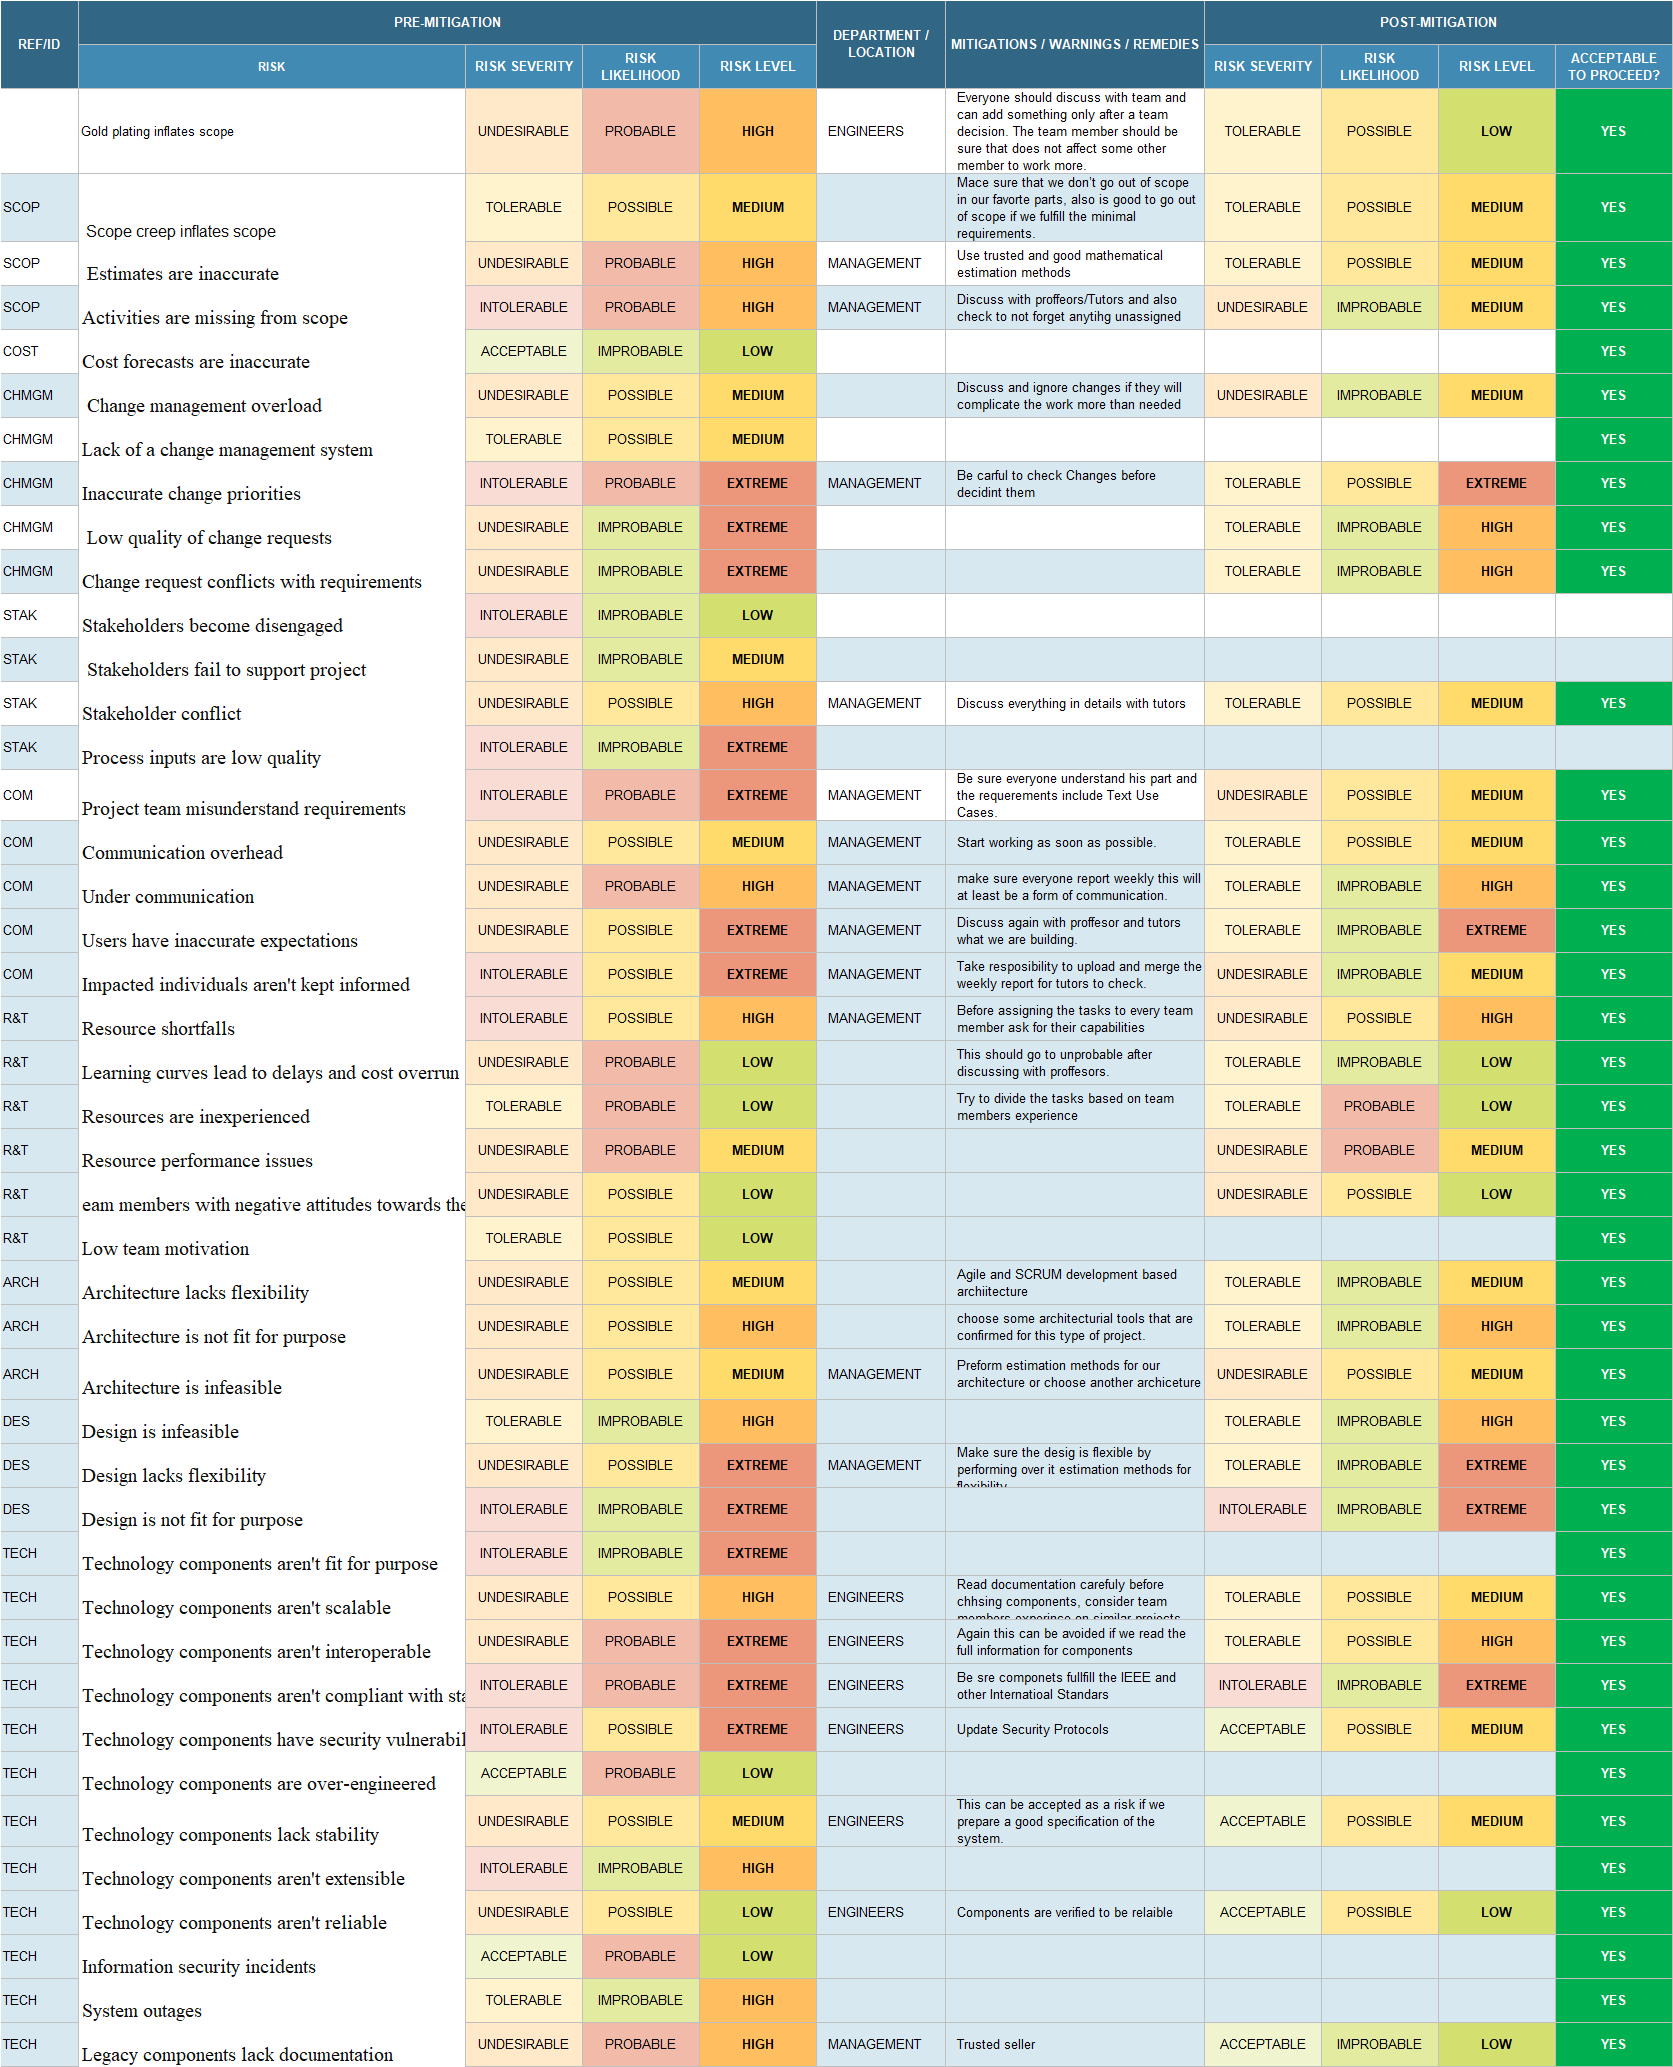
\includegraphics[scale=0.39]{images/Risk_Man_Matrix.png}
	\caption{Risk Management Matrix}
	\label{img:Risk_Man_Matrix}
\end{figure}
\FloatBarrier

\clearpage

\FloatBarrier
\begin{figure}[!h]
	\centering
	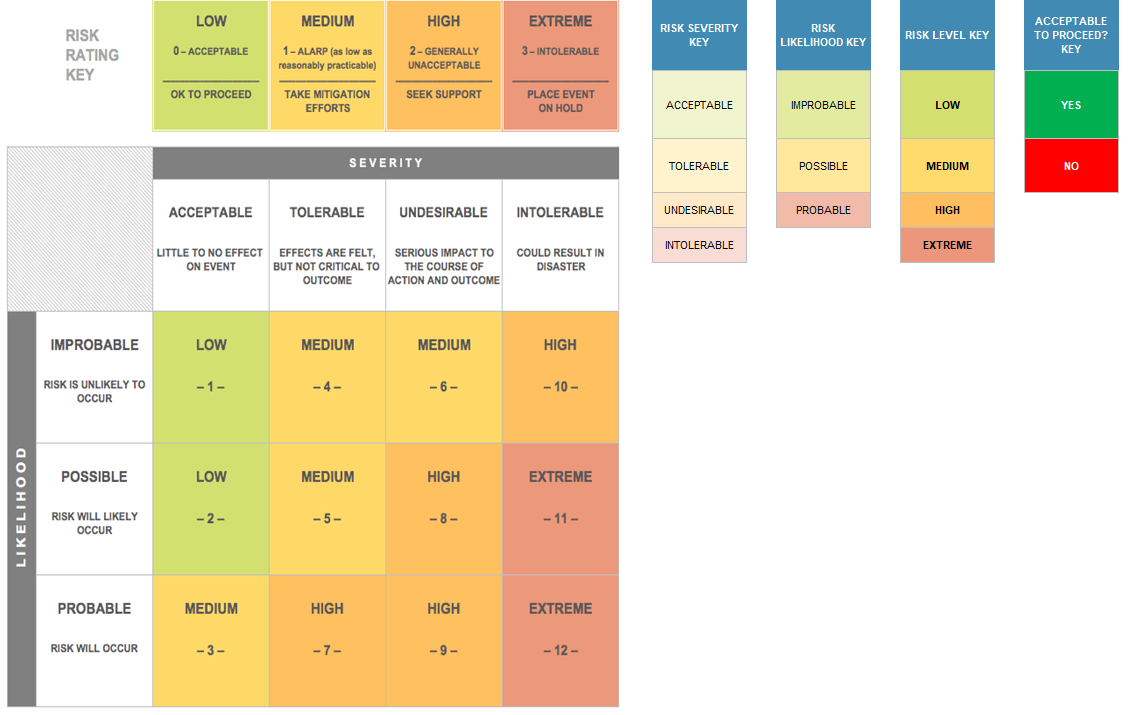
\includegraphics[scale=0.5]{images/Risk_Man_Key.png}
	\caption{Risk Management Matrix Key}
	\label{img:Risk_Man_Key}
\end{figure}
\FloatBarrier	

\section{Design}
\subsection{Use Case Diagram}

\textit{System Start}: User presses button on SensorTag to turn it on. PC app connects to SensorTag and starts receiving data\\
\textit{Recognises Fall}: User falls, system recognizes fall and requests help\\
\textit{Receiving False Alarm}: User “falls”, system recognizes fall and receives False Alarm signal\\
\textit{Personal data changes}: User modifies his personal data and system saves changes\\
\textit{Calibration changes}:  User modifies calibration and system saves changes\\\\\\\\\\\\\\\\\\\\\\\\\\\\\\\\\\\\\\

\FloatBarrier
\begin{figure}[!h]
	\centering
	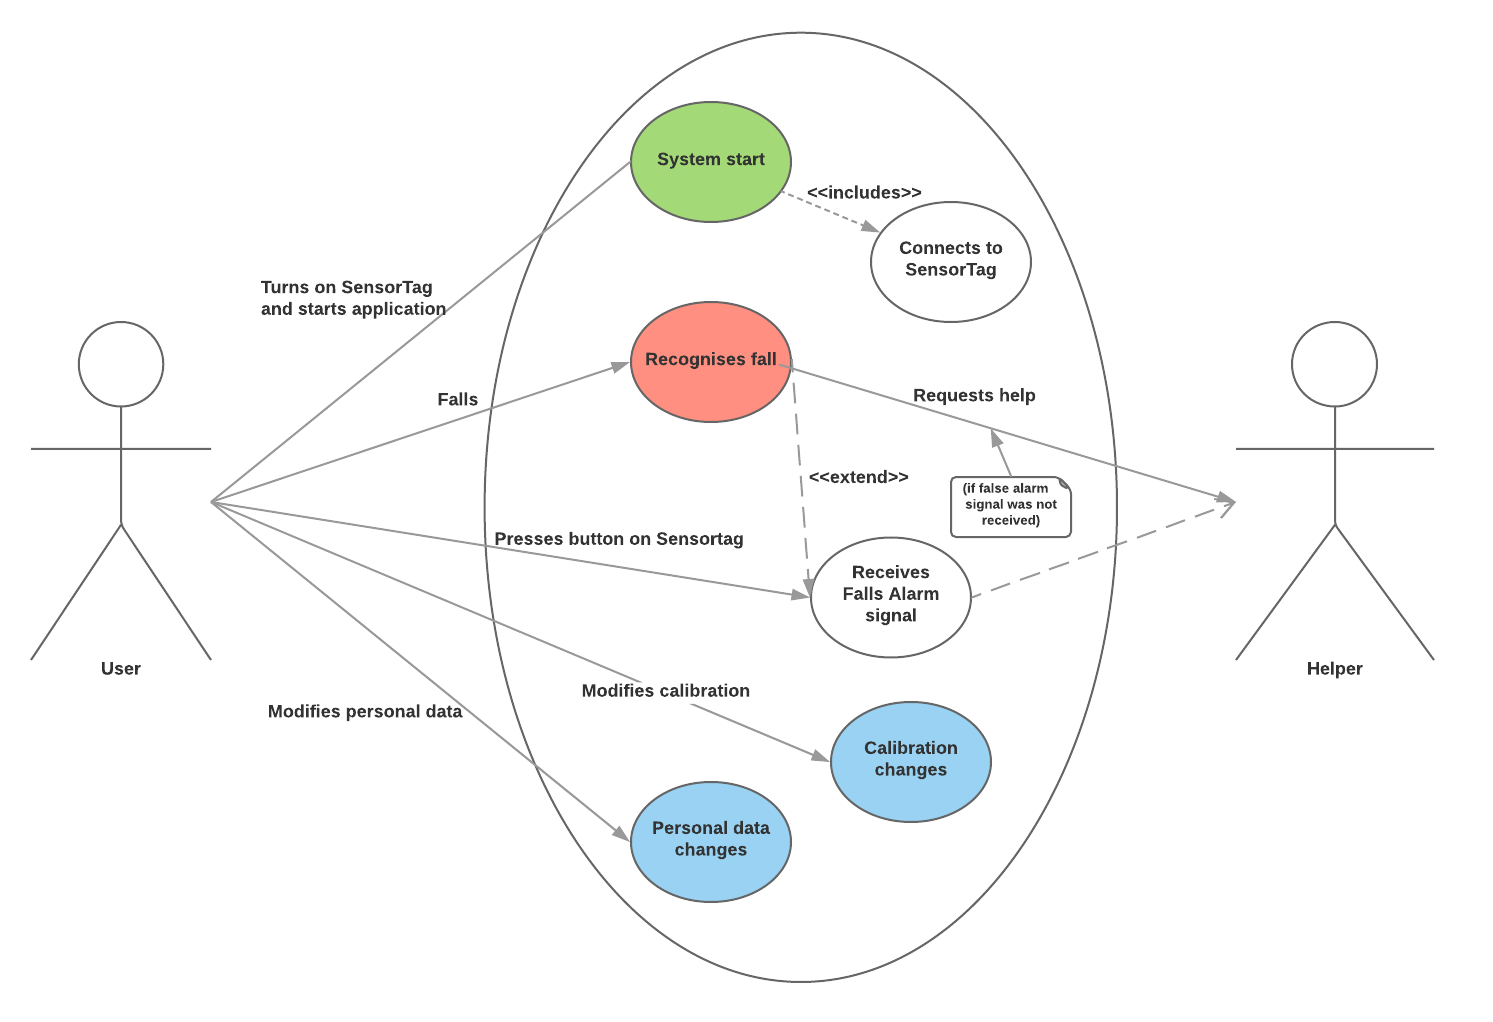
\includegraphics[scale=0.23]{images/Use_Case_Diag.png}
	\caption{Use Case Diagram\textsuperscript{\cite{umlspec}}}
	\label{img:Use_Diag}
\end{figure}
\FloatBarrier

\subsection{Sequence Diagrams taken from the Use Cases}
To better clarify the Use Case diagram, we included below the following sequence diagrams concerning the most complicated parts.

\FloatBarrier
\begin{figure}[!h]
	\centering
	\caption{System Start}
	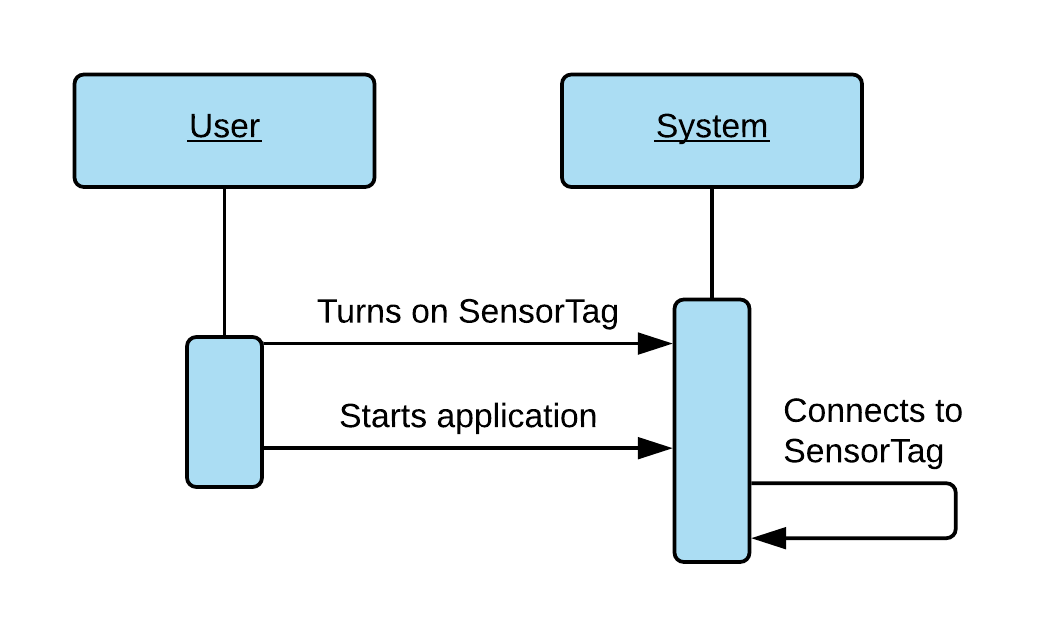
\includegraphics[scale=0.25]{images/Seq_Sys_Start.png}
	\label{img:start}
\end{figure}
\FloatBarrier
\FloatBarrier
\begin{figure}[!h]
	\centering
	\caption{Recognize Fall}
	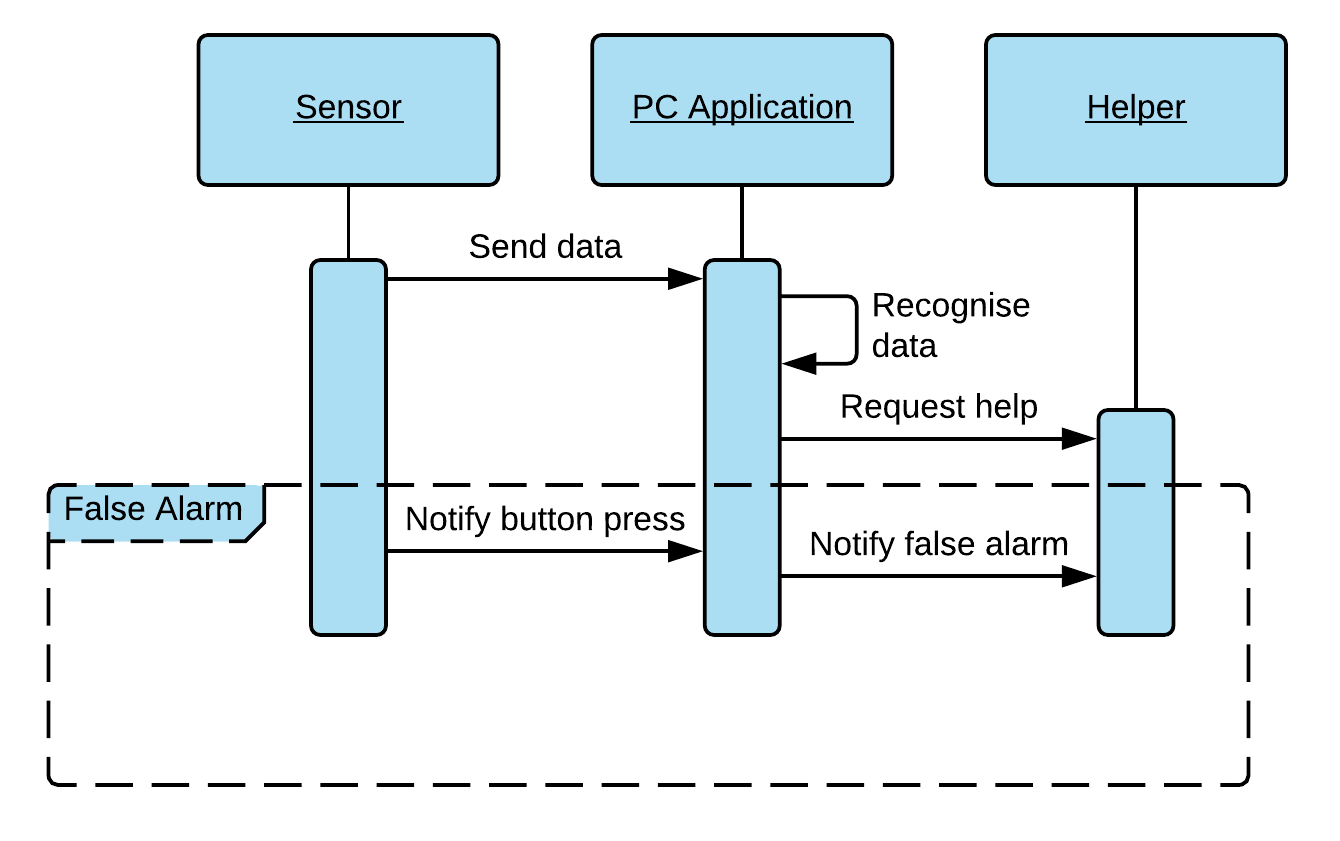
\includegraphics[scale=0.2]{images/Seq_Rec_Fall.png}
	\label{img:recfall}
\end{figure}
\FloatBarrier

\subsection{Architecture}
The system consists of two TI Sensortags connected via Bluetooth LE to a TI Launchpad, which is in turn connected via USB to a PC. Initially, in an effort to simplify the development, we intended to connect the Sensortags directly to a BLE enabled PC. However, that turned out to be more difficult than expected and it was therefore decided to use a Launchpad to interface the two.\\
Each Sensortag runs a slightly modified version of the original TI application "\textit{sensortag\_cc2650stk\_app}": they gather data through their built-in sensors and send it over BLE to the Launchpad. In this BLE connection, the Sensortags act as peripheral devices, while the Launchpad as the central device.\\
The Launchpad runs an unmodified version of the TI firmware\textsuperscript{\cite{hosttest}}. It receives the sensor data and makes it available to the PC application through a USB COM port.\\
The PC application analyses the sensor data stream to detect fall events. Then, if necessary, it notifies the helpers that the user has fallen. The PC application possesses a GUI where the sensor data is used to display graphs. Additionally, the GUI can be used to calibrate the fall detection algorithm, and to change the stored user and helper personal data.\\
The diagram below shows the main system component:
\FloatBarrier
\begin{figure}[!h]
	\centering
	\caption{Component Diagram}
	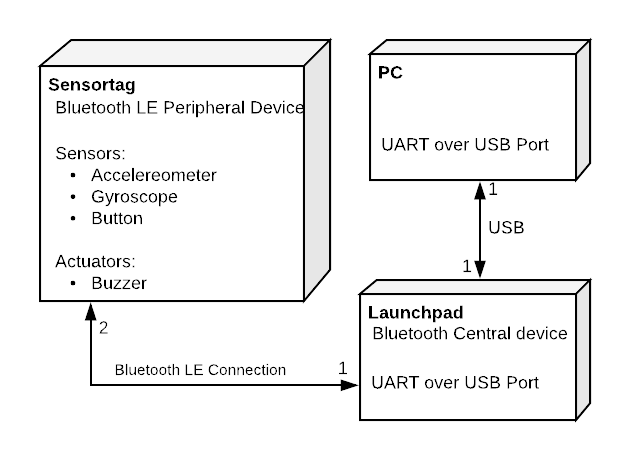
\includegraphics[scale=0.4]{images/Comp_Diag2.png}
	\label{img:compdiag}
\end{figure}
\FloatBarrier

\subsection{Software Architecture}
Our application has six main classes, which will be explained further below.\\
The Server class represents the open COM port operations. This class not only opens the port, in order to allow the application to perform operations, it also handles the reads and writes to the port. This is a Singleton class, so we do not create a new instance by mistake and try to open the port again, as that will result in an exception.\\
The Mathems class is the Fall Detection Algorithm. It is also a Singleton class, because it is a different thread that tries to access resources on the Server. If we create two instances, we risk running into deadlocks.\\
Server class and ProcessMessage read and translate the messages for our application. FallNotificationService is the class that will send the email and notify the helper for a fall or a false alarm.\\
How these classes communicate and work together is described by these sequence diagrams.

\clearpage
\FloatBarrier
\begin{figure}[!h]
	\centering
	\caption{UML Diagram}
	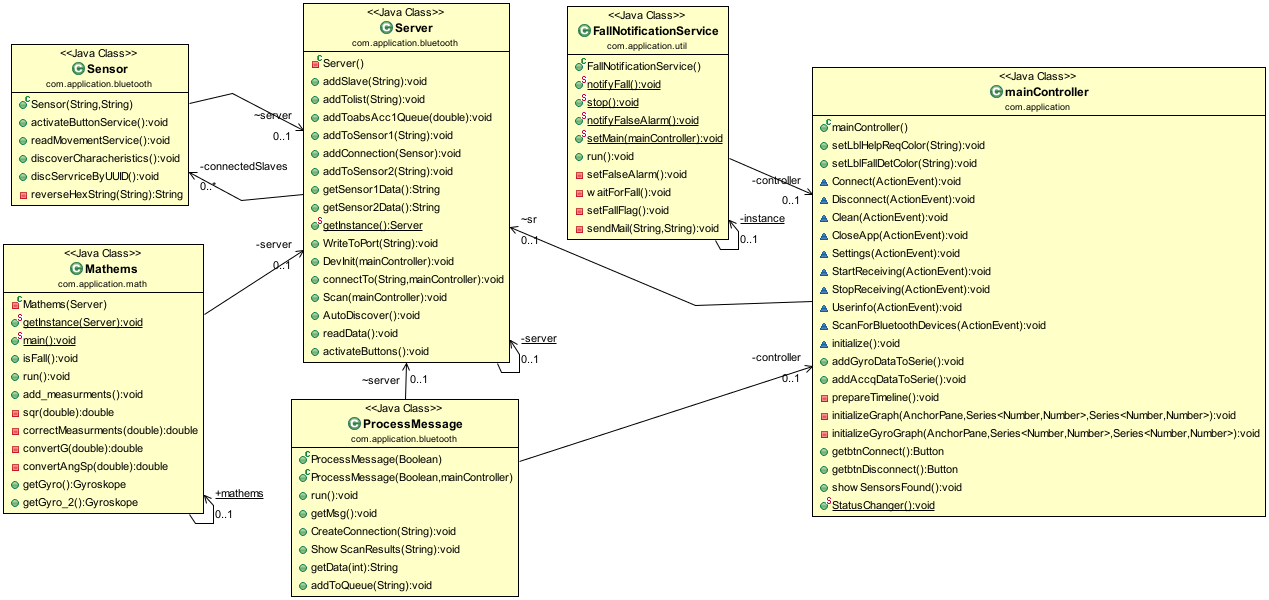
\includegraphics[scale=0.4]{images/UML_Diag.png}
	\label{img:UML_Diag}
\end{figure}
\FloatBarrier

\FloatBarrier
\begin{figure}[!h]
	\centering
	\caption{Fall Detection Sequence Diagram}
	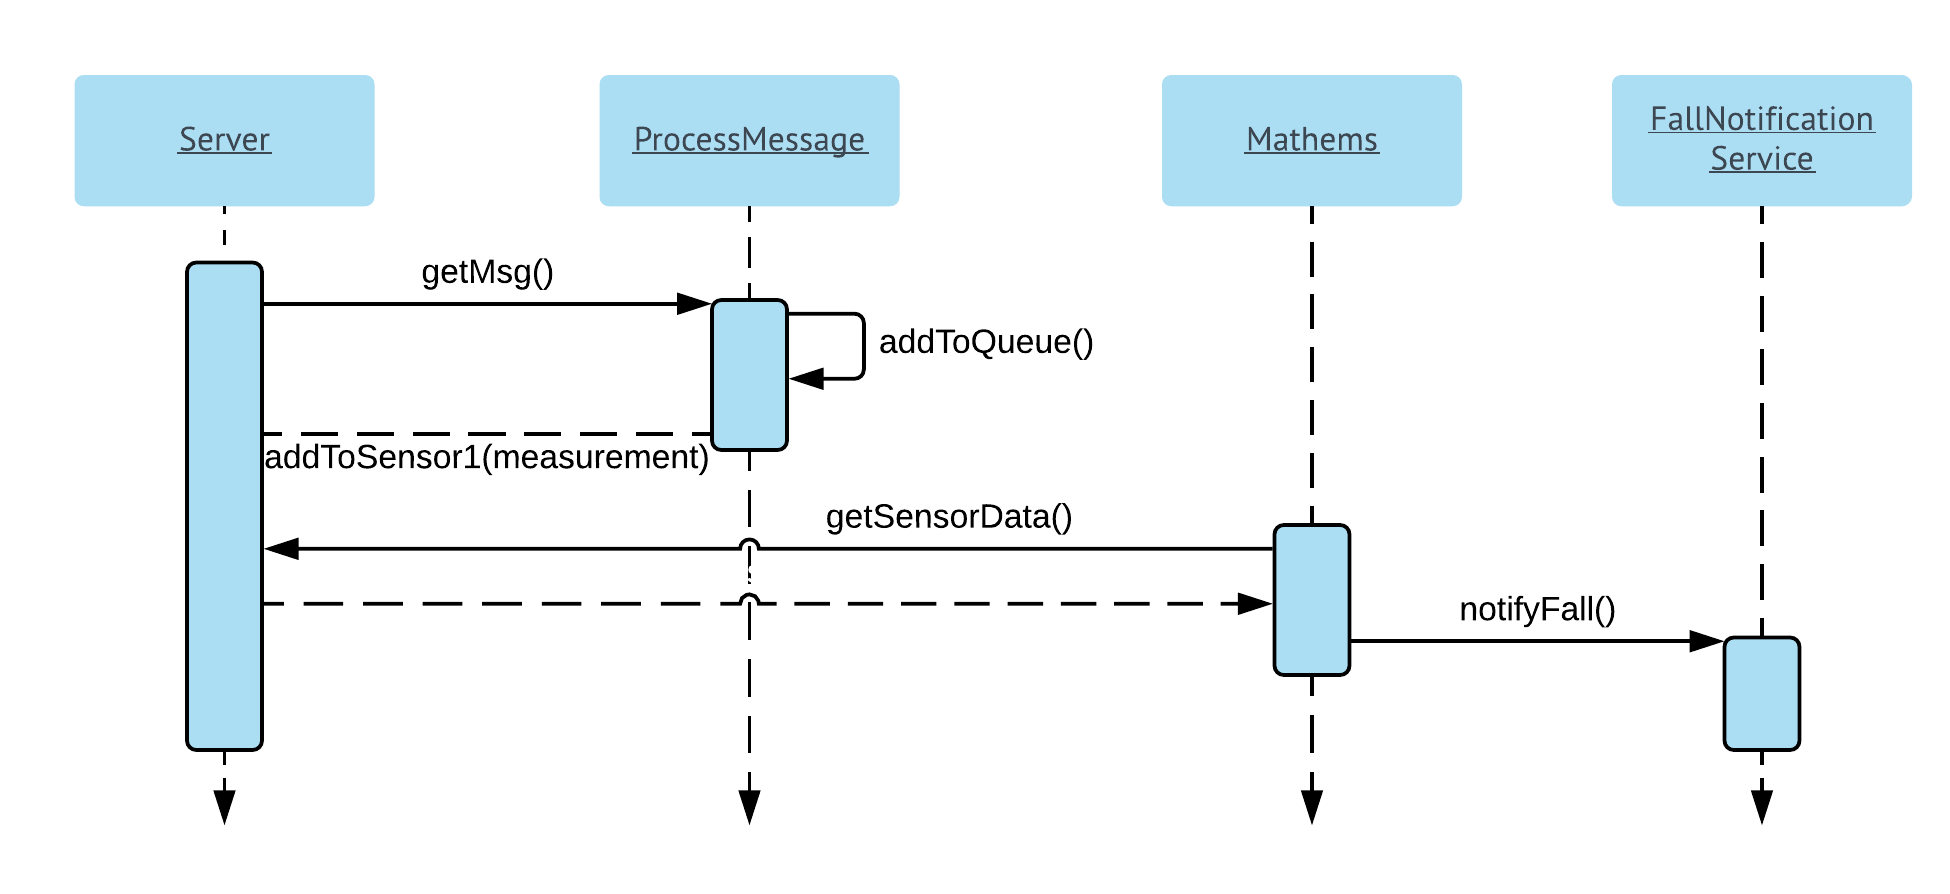
\includegraphics[scale=0.55]{images/Seq_Fall.png}
	\label{img:fall}
\end{figure}
\FloatBarrier

Server will tell the ProceessMessage that we have a new data, ProcessMessage will check if it measurement and if yes will save them to the Server. Mathems will analyze the measurements and if it is a Fall will tell FallNotificationService to send for help.

\FloatBarrier
\begin{figure}[!h]
	\centering
	\caption{False Alarm Sequence Diagram}
	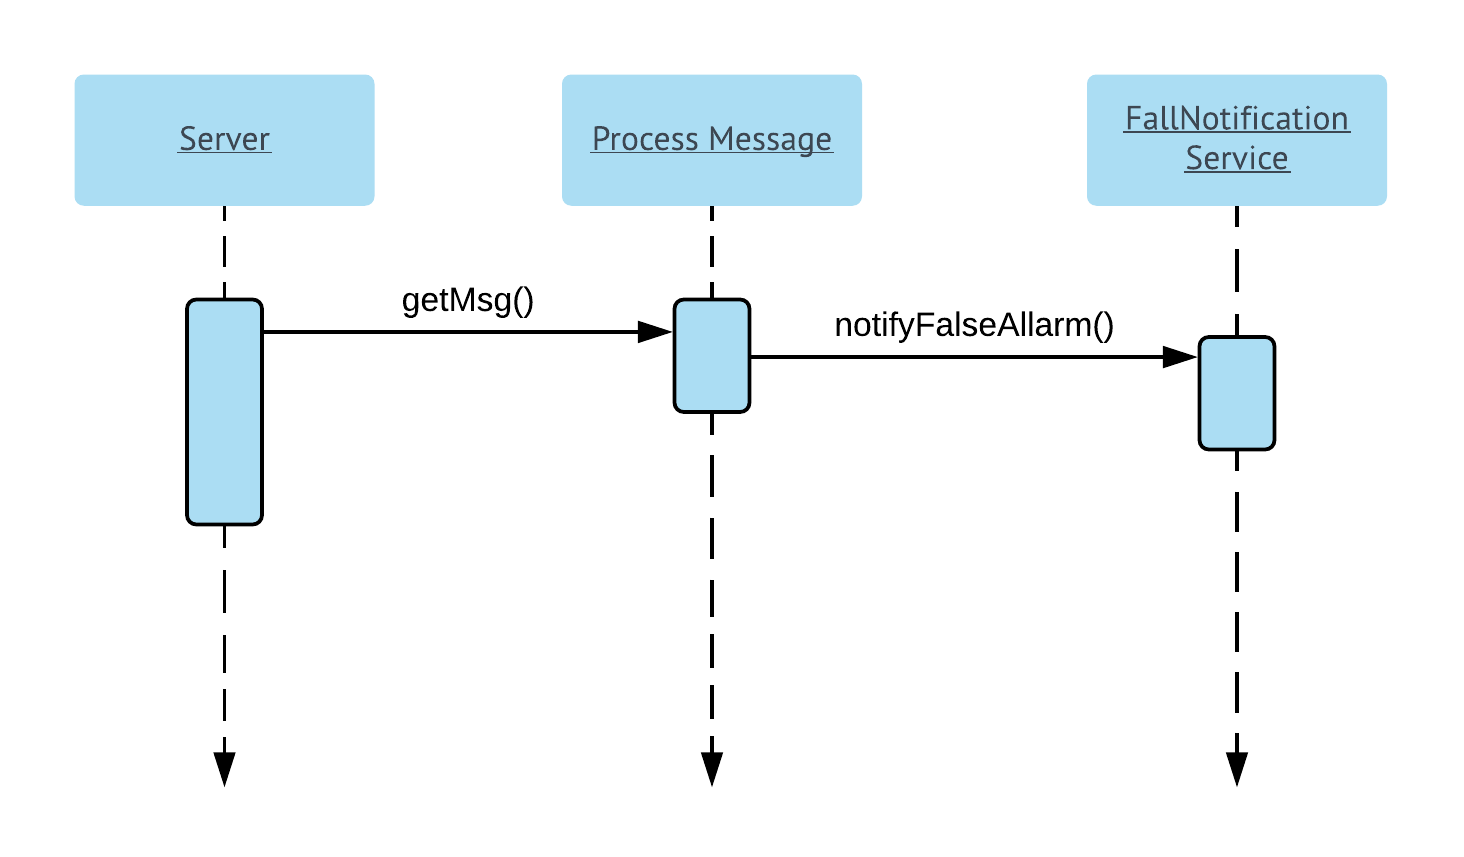
\includegraphics[scale=0.43]{images/Seq_FalseAl.png}
	\label{img:falseal}
\end{figure}
\FloatBarrier
\hskip 1cm \\\\\\\\\\\\\\\\\\\\\\\\\\\\\\\\\\\\
When the Server object gets new data it asks the ProcessMessage to find out what message that was. If it was a message from I/O service it means that the button on the SensorTag was pressed and will notify that the previous alarm was a false one.

\FloatBarrier
\begin{figure}[!h]
	\centering
	\caption{Connecting to Sensor}
	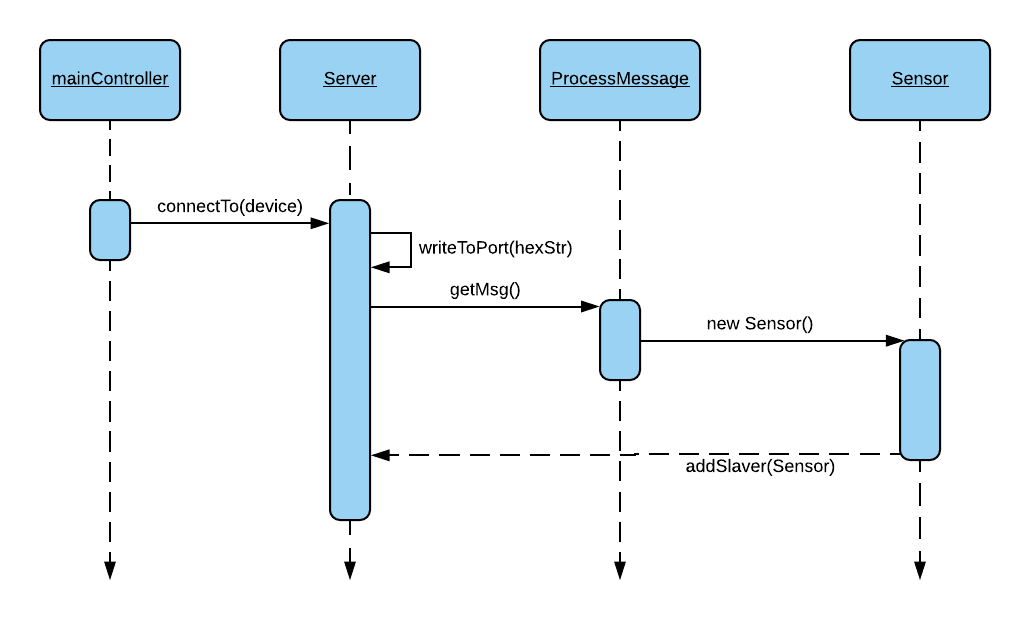
\includegraphics[scale=0.5]{images/Seq_Slav_Conn.png}
	\label{img:slav}
\end{figure}
\FloatBarrier
Here we see also the main controller class that works like a bridge to send commands from the GUI to the backend. From GUI we ask the Server to connect to a device. The Server object will write to the COM port, which is the bridge between our application and Launchpad. After receiving a response from the Launchpad, the Server will ask the ProcessMessage to translate the message received, and if it is the comfirmation message for a new slave connected to the master, it will create a new object of type Sensor and will add the reference to the Server.

\subsection{Technologies, Libraries, IDEs, Tools}
Technologies used for this appliation are Java as a programming language for backend development, JavaFX for GUI Development. Gradle as a build tool, java-simple-serial-connector\textsuperscript{\cite{javasimpconn}} library for reading  a serial port in java. The ObjectAid UML Explorer for Eclipse\textsuperscript{\cite{ojectaid}}, Eclipse IDE. C programming Language for Sensor Tags. \LaTeX \space for Documentation.

\section{Measurement Chain\textsuperscript{\cite{prodspec}}}
The application makes use only of the MPU-9250 sensor pack present on the Sensortags, which includes a three-axis accelerometer, a three-axis gyroscope and a three-axis magnetometer (the last is not used and was deactivated).\\
The \textit{measuring object} is the sensor itself (the acceleration and orientation of it). Since it is rigidly mounted on the PCB, we can assume that corresponds to measuring the movement of the whole Sensortag. However, we cannot ignore the soft connection of the Sensortag to the belt and of the belt to the user. This requires adaptation of the fall detection algorithms to many different user/clothing combinations (which is achieved by means of the calibration constants accessible through the GUI).\\
The \textit{measured quantities} are: the total resulting acceleration (gravity plus motion) on each axis; the angular velocity on each axis.\\
The \textit{measurement method} is indirect (see individual sensor description below).\\\\
The complete \textit{measurement chain} consists of the sensors themselves, the ADCs built into the MPU-9250, and the number conversion that takes place in the desktop part of the application. Since the signals are transmitted only after the analog to digital conversion takes place, we don’t have to worry about signal degradation due to analog transmission.

\subsection{Accelerometer}
"The accelerometer uses separate proof masses for each axis. Acceleration along a particular axis induces displacement on the corresponding proof mass, and capacitive sensors detect the displacement differentially." The analog value is digitalized by three 16bit sigma-delta ADC (one per axis). The resulting value may be written as:
$$ a = val \pm e_i \pm e_T \pm e_l \pm e_{cal} \pm e_n \quad g $$
Where \textit{val} is the real value, $e_i$ is the intrinsic error (3\%), $e_T$ is the temperature induced error (0.026\%/$^{\circ}$C), $e_l$ is the non-linearity error (0.5\%), $e_{cal}$ is the initial calibration error (80 mG) and $e_n$ is the noise (8 mG). At room temperature and for the threshold values used by our fall detection algorithm, the above formula can be approximated with:
$$ a = val \pm 6\%  \quad g $$

\subsection{Gyroscope}
The gyroscope’s sensors consist of 3 vibratory MEMS. "When the gyros are rotated about any of the sense axes, the Coriolis Effect causes a vibration that is detected by a capacitive pickoff." The resulting value may be written as:
$$ v_{ang} = val \pm e_i  \pm e_T \pm e_l \pm e_{cal} \pm e_n \quad ^{\circ}/s $$
Where val is the real value, $e_i$ is the intrinsic error (3\%), $e_T$ is the temperature induced error (4\%), $e_l$ is the non-linearity error (0.1\%), $e_{cal}$ is the initial calibration error (5 $^{\circ}/s$) and $e_n$ is the noise (0.1 °/s). At room temperature and for the threshold values used by our fall detection algorithm, the above formula can be approximated with:
$$ v_{ang} = val \pm 9\% \quad ^{\circ}/s $$


\section{Fall Detection Algorithm}
The Fall Detection Algorithm is the back end logic of the application, where the application handles decisions about a fall. The logic is divided into several parts, each of which is responsible for its own goals and tasks. It contains three classes:
\begin{itemize}
	\item Mathems class - contains main thread of computations, creating stamp of Gyro and Accelerometer objects inside the thread, and contains main static variables like impact power, laying acceleration;
	\item Gyroscope class - contains measurements from sensor, functions of adding new measurements, thread of Gyro computations;
	\item Accelerometer class - contains measurements from sensor, functions for adding new measurements, can trigger Gyro method to start its thread.
\end{itemize}
It is better to start discovering parts of data from end to beginning. The "Gyroscope class" stores queues for every axis of its measurements, the logic of the calculation degrees, which were made during the fall, the functionality of adding new measurements into the queue and a link to the "Mathems class". The "Accelerometer class" contains queues for every axis of its measurements, the logic of calculation impact, meaning the impact which is made at contact with the floor, the functionality of adding new measurements into the queue, finding the beginning of the fall, checking if the patient is still laying on the floor and a link to the "Mathems class". The main part, which is called "Mathems class", contains the main thread of mathematical computations, with two pairs of objects: Gyro and Accelerometer for each SensorTag, the object Server, and several flags to inform about the fall. Also, it has the functionality of adding, parsing and converting measurements which come from the SensorTags.

\subsection{Configuration Storage}
The class of Configuration Storage was made to store all the static variables, which are used through all the application. It is an abstract and static class, which is why the application can have access to the variables from everywhere without having an instance of its object. The main aim of this class is to store main static values in one place. Furthermore, all static variables in the class have get()/set() methods and are connected to the UI, which gives it the advantage of changing them without restarting the application. For example, if an expert user wants to change the value of the impact, they can change it in "Settings" window.

\subsection{Main Thread and Work Logic}
The "Mathems class" was implemented as a class, which extends the Thread class, and it uses the Singleton pattern to have only one instance of the object. It was done this way because the object should be created only when the SensorTag sends values. In the constructor of the class, the application starts the main thread of the Mathematical model. The main tasks of the mathematical model execute only in this thread.\\
First of all, the main thread asks the Server for new measurements from SensorTags. If there is no new values then the thread will wait for $10ms$. Then, the thread has a fork: either add new measurements if the queue is less than the $ConfigurationStorage.getSKIP\_MEASURE()$ static variable, or make computations of the fall if there is enough measurements.\\
On the first few weeks of the project, it was calculated by the kinematic equation:
$$ \vartriangle x = v_0t + \frac{1}{2}at^2 $$
minimum amount time which is need for the fall. The sensor falls from \textit{1m} high. This means that the minimum fall time will be \textit{450ms}. In addition, Raul Bertone increased the speed of the output measurements from the SensorTag; now we get 20 measurements per second, which means that the application gets measurements every \textit{50ms}. Consequently, for calculations it should store at least 10 measurements per one timeframe. Unfortunately, after several tests it was stated that the application should store more values because the amount is too small to distinguish the fall. Now there are 20 values for calculations and 10 from the past timeframe.\\
The function $add\_measurments$ asks the Server for new measurements, then converts them for G and Degree velocity scale. Finally, it adds them into the graph and the corresponding queues for the Gyroscope and the Acclerometer\textsuperscript{\cite{movsens}}.\\
Furthermore, the class has two flags for the fall: $isAclrFall \&\& isGyroFall$. The Gyroscope and the Accelerometer classes change their values. They are checked by the thread every pass. If they are both "\textit{true}" the thread calls $FallNotificationService.notifyFall()$. It creates a notification of the fall.

\subsection{Accelerometer}
Every pass of the tread triggers the method $isArclFall$ to start calculations of the Accelerometer. The method makes a copy of objects every time it is triggered and starts in a loop to calculate the absolute value of the impact of all the axes together for every measurement.
\begin{center}
	$impact = \sqrt{Gx^2 + Gy^2 + Gz^2} > 2,$
	$where \quad \textit{Gx, Gy, Gz} \quad are \quad axis $ \\
	$values;$
\end{center}
If the impact is more than $2g$ it is going to check if the patient is laying to be sure that it was a fall. The Laying function skips several measurements after impact to be sure that the patient is in a static position. If the absolute value on OX and OY axis is between 0.8 and 1.3 it means that patient is laying.
$$ 0.8 < \sqrt{Gx^2 + Gy^2} < 1.3 $$
If the patient is laying, the application changes the first flag that a fall was detected from the Accelerometer. Then the class calls the method of the Gyroscope class to calculate the change in degrees that was registered by patient during the fall. To do this, the Accelerometer class should calculate when the fall starts. This is calculated by a function $getFallStart$. The function takes the index of the impact values, subtracts five measurements back and starts one by one to check when the last absolute value on the OZ axis between 0.8 and 1.3 was. This way the application can understand the last index of the measurements when the patient was standing.
$$ 0.8 < \left|Gz\right| < 1.3 $$

\subsection{Gyroscope}
To use only the Accelerometer is not enough to prove that it is a fall. The application should include protection from making wrong decisions. That is why it was important to implement the additional logic of the Mathematical package.\\
The application should store data from the sensors for the Gyroscope the same way as for the Accelerometer class in parallel. Then, the Gyroscope starts to calculate the degrees on OX and OY axes, which were registered by the patient between the beginning of the fall and the impact indexes. \\
The class has only the degrees' velocity (degrees per second), which is why the application should convert them into actual degrees. The conversion for every measurement can be made by dividing the speed with the amount of values per second. Then the application should sum up all the values from the beginning of the fall till the impact.\\
\begin{center}
	$angle_i = \left| \frac{Gx_i}{CS} \right| + \left| \frac{Gy_i}{CS} \right|,$\\
	$where \ Gx,\ Gy\ is\ the\ velocity\ on\ OX\ and\ OY\ axis;$ 
	$CS\ is\ the\ amount\ of\ measurements\ per\ second;$
\end{center}
Then this value should be divided by 180 and the application should take the remainder of the division and subtract from it 90 degrees. If this value is less than 30 degrees the application changes another flag for "true".
\begin{center}
	${\sum}_i angle_i - 90 \pm 180 * n < 30,$ \\
	$where \quad n \in Z; $
\end{center}

\subsection{Problems}
The main thread work continuously that is why during computations the application could link on the values in the queue, which have been changed. It can bring errors in logic of work. That is why the application make copies of objects of the Accelerator and Gyroscope classes.\\
Another one problem was connected to the creating only one instance of the "Mathems class". It was stated that the main thread should be created only when the first values come from the SensorTags. That is why instance of the class is implemented by Singleton pattern and the application creates it in the Server class.\\
One of the main problems was with detecting a fall when the patient falls on the first measurements of the queue. Because the application cannot go back in measurements to detect when the fall was started. That is why the Accelerator and Gyroscope objects store 30 measurements. However, first 10 measurements do not use in impact calculations. They are used in calculation of finding last horizontal position of the patient.\\
Finally, the application skips first five measurements when it is trying to find last horizontal position. It is made because after fall patient can have some noise. That noise can be detected as last horizontal position but it is not true.

\section{Development}
\subsection{Sensortags}
As a base for development, we made use of the "\textit{sensortag\_cc2650stk\_app}" TI project, to which we made the modifications described below.\\
\textit{Feature activation and deactivation}: since our project only makes use of the accelerometer and gyroscope, we choose to turn off all the other sensors. To do this, we used the TI preferred method, i.e. the "\textit{EXCLUDE}" pre-processor directives. For a complete list of the employed directives, please see [\citetitle{2ndreport}]. In the same way we also activated the buzzer.\\
\textit{Movement sensor configuration}: using the appropriate bitmask in the \textit{mpuconfig} variable, we were able to configure the set the sensitivity of the accelerometer to +/- 4g and turn off the magnetometer.\\
\textit{Update rate}: we increased the update rate of the whole sensor to 20Hz (instead of the standard 1Hz).\\
\textit{I/O service}: to be able to control the buzzer remotely via Bluetooth, it was necessary to modify the I/O service configuration, setting it to its "remote" mode.

\subsubsection{Problems with Sensortags}
Sometimes our Sensortags would stop working after flashing. We found out that, on some computers, after flashing by connecting the debugger module via USB 3.0 the Sensortag would then only work while powered through the Debugger itself, but not on battery alone. To avoid this, it was enough to flash via a USB 2.0 port instead of 3.0. However, to repair a Sensortag  that already been flashed over USB 3.0, it was first necessary to flash the hex file using the Flash Programmer 2 (again, only via USB 2.0).\\\\
With an early version of our modified firmware, the data stream coming from the Sensortag would freeze every few seconds, only to resume shortly thereafter. After talking with Group 2, which made similar modifications but didn’t use the "EXCLUDE" directives for the pre-processor, we were mislead into thinking that the directives themselves were at fault. This made us lose some time chasing a red herring. Debugging revealed however that the “bug” was actually a feature we inadvertently turned on, namely  Wake-On-Motion. This interrupts the sending of sensor data when there is no movement for more than a few seconds. Turning the feature back off, neatly solved the problem.

\subsection{Desktop Application Development}
\subsubsection{Problem with Connecting 2 SensorTags to the Application}
Since SensorTags were configured and implemented as slaves we need a bluetooth profile as a server. For that we had different possibilities. First, we decided to develop a bluetooth profile directly on a Laptop device but there was no support or lib for that in Windows. All we could find was the Tinyb\textsuperscript{\cite{tinyb}} project, which would work only under Linux and could be adapted for Windows implementing the Bluetooth profile in C++ then using JNI to use the code on our Java application.\\\\
The other possibilities were using a smart phone as a master device. We tried to do that in Python but from the lack of experience of our team in this programming language we decided to use a Launchpad, something that until then we were trying to avoid using because the Launchpad was a black box for us. Nevertheless, that was the final solution we decided on. Now the problem was how the Launchpad would communicate with the computer.\\
Windows recognizes the Launchpad as a serial port and we need to use that serial port to transfer messages between our application and Launchpad. For that we use jssc\textsuperscript{\cite{javasimpconn}} library to open port and to Read and Write from that. This way we could write and read byte arrays to the port perfectly. We could also exhange messages with the master Bluetooth profile.

\subsubsection{Deciding What to Send to the Launchpad}
We used the help of BTool from the core TI applications. From there we could find the hexadecimal string to advertise the Launchpad, scan for discoverable bluetooth devices and connect to a desired one.\\
The problem now became how to read and translate the messages, the byte arrays we get from COM serial port.\\
From the documentation of TI Bluetooth profile\textsuperscript{\cite{vendor}} we found out that a new message from the Launchpad to the serial port always starts with the hexadecimal value of 0x04FF, then we used the TI Documentation to find out what the rest of the message means.\\\\
Another problem was that the serial port in Windows can read only 8 bytes at a time and the messages for Launchpad were much longer, so there we had a problem where we receive a new 8 byte array, and we check if the first 2 bytes are 0x04FF. After that next bit was the length of the message, which is mainly where the problem lay. Lets suppose we receive the message 04FF0C010600010000 690153036C53\\
What this message means is displayed in Figure \ref{img:msgstruct}.\\
What we were reading from our application is the following:\\
04FF0C010600010000\\
690153036C53..next message.\\
Whenever we have a new array we check if it starts with 0x04FF. Then we need 0x0C =12 bytes for the data length but we have only 5  bytes left from the array before we get the next array so the message can be misinterpreted.
\FloatBarrier
\begin{figure}[!h]
	\centering
	\caption{Message Structure}
	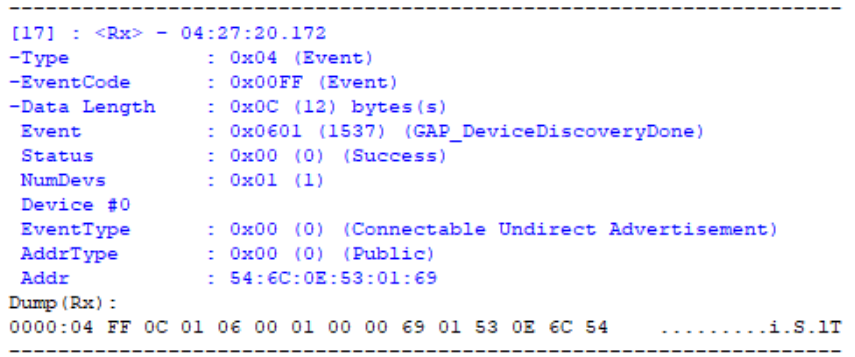
\includegraphics[scale=0.3]{images/msgstruct.png}
	\label{img:msgstruct}
\end{figure}
\FloatBarrier
To solve this we put everything that we get from the Launchpad in a byte queue then we create a new thread just to process that queue and read the messages. We read only the messages that we need and the others we just ignore.

\subsubsection{Fall Notification Service (FNS)}
This is the service that handles the notifications triggered by the detection of a fall. Its code interacts with each and every other part of the desktop application and offers a good overview of its main features.\\
On start the FNS idles while waiting for a trigger. When the fall detection algorithm thinks the user has fallen, it alerts the FNS which turns on the buzzer in the Sensortag and raises the "Fall Detected" flag in the GUI and then waits for a preset amount of time (default 10 seconds) for feedback from the user in the form of a button press on the Sensortag. If no such feedback comes, help is requested (an email is sent to the helper’s address) and the "Help Requested" flag is raised in the GUI. Instead, in case a button is pressed before the preset time has elapsed, the buzzer is turned off and the "Fall Detected" flag lowered, after which the cycle repeats itself. The user can also signal a false alarm after help has been already request (that is, when in the "Wait" state): in this case, the buzzer is turned off, all flags are lowered and a new message is sent to the helpers explaining that it was indeed a false alarm.\\
Below you see a state machine diagram illustrating the service operation:
\FloatBarrier
\begin{figure}[!h]
	\centering
	\caption{Fall Notification Service}
	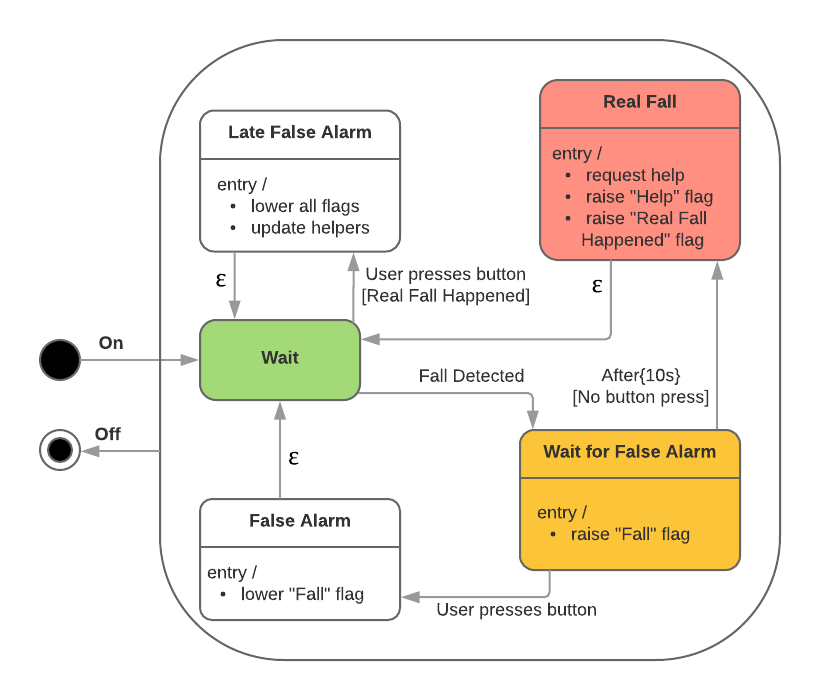
\includegraphics[scale=0.3]{images/FNS.png}
	\label{img:FNS}
\end{figure}
\FloatBarrier
The content of the messages sent to the helpers, as well as the addresses of the helpers themselves, can be changed through the GUI. The waiting time after a fall is detected and before help is requested, can also be modified in the same way.


\subsection{Graphical User Interface} 
To implement GUI based on the mock up made earlier, JavaFX Scene Builder\textsuperscript{\cite{JavaFX}} was used. JavaFX Scene Builder is a tool that lets users design a JavaFX application’s UI. UI components can be
draged and dropped to a work area, modify their properties and at the end we will have FXML code
for the created layout generated automatically. The result is a FXML file that can be combined with a Java project by binding the UI to the applications logic.\\
In the first version of GUI we have main window with area for Accelerometer and Gyroscope graphs
and buttons to establish and control the connections to the SensorTags.\\
Through the File menu the user can access the User General Information and Settings windows.
In User General Information the user should fill in the form with his data and the contact person‘s data.\\
In Settings menu the calibration values for the fall detection algorithm can be inserted.

\nocite{*}
%----------------------------------------------------------------------------
% Bibliography
%----------------------------------------------------------------------------	
\printbibliography
\end{document}
%----------------------------------------------------------------------------
